\section{TacoTron}
\paragraph{Authors:} Yuxuan Wang,\dots , Rob Clark, Rif A. Saurous \cite{wang_tacotron_2017}


\subsection{Problem to solve}
End2End Text-To-Speech is a remaining frontier for ML systems, typically requiring extensive in-subject technical knowledge to set up. 
The goal of a end2end TTS system that can model \(p(\mathtt{Audio}|\mathtt{Text})\) directly, is therefore very useful. 
The main issue here, is that TTS encompasses an \textit{Inverse Problem}, i.e. a problem where the input dimensionality is much LOWER than the output dimensionality. 

Tacotron is proposed as an integrated end-to-end generative TTS model that takes a character sequence as input and outputs the corresponding spectrogram. 

\subsection{Architecture}
\begin{figure}[h!]
    \centering
    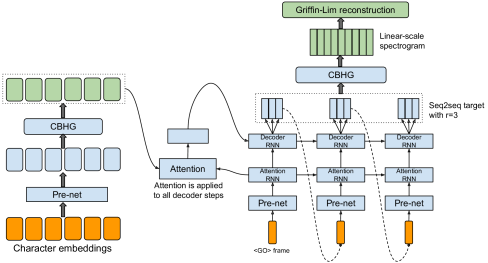
\includegraphics[width=\textwidth]{figures/tacotron-arch.png}
    \caption{Overall architecture of TacoTron TTS system. 
    The CBHG module is described in \cref{fig:tacotron-cbhg}}
    \label{fig:tacotron-arch}
\end{figure}


\paragraph{Convolution Bank + Highway Net + Bidirectional GRU feature}
(CBHG) consists of a bank of 1-D convolutional filters, followed by highway networks and a bidirectional gated recurrent unit (GRU). 
The input sequence is first convolved with 
\(K\) sets of 1-D convolutional filters, where the $k$-th set contains $C_k$ filters, like modelling unigrams, bigrams, \dots $K$-grams.  

Convolution outputs are fed into a multi-layer highway network to extract high-level features. 
Finally, we stack a bidirectional GRU RNN on top to extract sequential features from both forward and backward context.

See \cref{fig:tacotron-cbhg} for a visual.

\begin{figure}[h!]
    \centering
    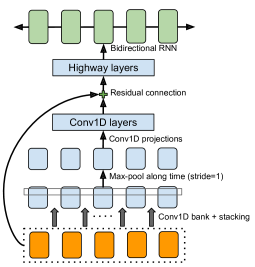
\includegraphics[width=0.55\textwidth]{figures/tacotron-cbhg.png}
    \caption{The CBHG module in the TacoTron architecture. }
    \label{fig:tacotron-cbhg}
\end{figure}

\paragraph{The Encoder} 
on the left side of \cref{fig:tacotron-arch} passes the input character embedding sequence 
to a bottleneck layer and through a CBHG to an encoded representation of the entire sequence.  


\paragraph{The Decoder} consists of a 2-layer FC pre-net, an Attention GRU (RNN), and a Decoder stack of GRUs with vertical residual connections. 

